\begin{figure}[h!]
	\centering
	
	
	
	% Gradient Info
	
	\tikzset {_3sybf9svc/.code = {\pgfsetadditionalshadetransform{ \pgftransformshift{\pgfpoint{0 bp } { 0 bp }  }  \pgftransformrotate{0 }  \pgftransformscale{2 }  }}}
	\pgfdeclarehorizontalshading{_msh882t58}{150bp}{rgb(0bp)=(0.82,0.01,0.11);
		rgb(37.5bp)=(0.82,0.01,0.11);
		rgb(43.973214285714285bp)=(0.97,0.91,0.11);
		rgb(49.24107142857143bp)=(0.72,0.91,0.53);
		rgb(55.58035714285714bp)=(0.11,0.97,0.94);
		rgb(62.00892857142857bp)=(0.8,0.29,0.89);
		rgb(100bp)=(0.8,0.29,0.89)}
	
	% Gradient Info
	
	\tikzset {_s6rolseyi/.code = {\pgfsetadditionalshadetransform{ \pgftransformshift{\pgfpoint{0 bp } { 0 bp }  }  \pgftransformrotate{0 }  \pgftransformscale{2 }  }}}
	\pgfdeclarehorizontalshading{_2kvz2ka7v}{150bp}{rgb(0bp)=(0.82,0.01,0.11);
		rgb(37.5bp)=(0.82,0.01,0.11);
		rgb(43.973214285714285bp)=(0.97,0.91,0.11);
		rgb(49.24107142857143bp)=(0.72,0.91,0.53);
		rgb(55.58035714285714bp)=(0.11,0.97,0.94);
		rgb(62.00892857142857bp)=(0.8,0.29,0.89);
		rgb(100bp)=(0.8,0.29,0.89)}
	\tikzset{every picture/.style={line width=0.75pt}} %set default line width to 0.75pt        
	
	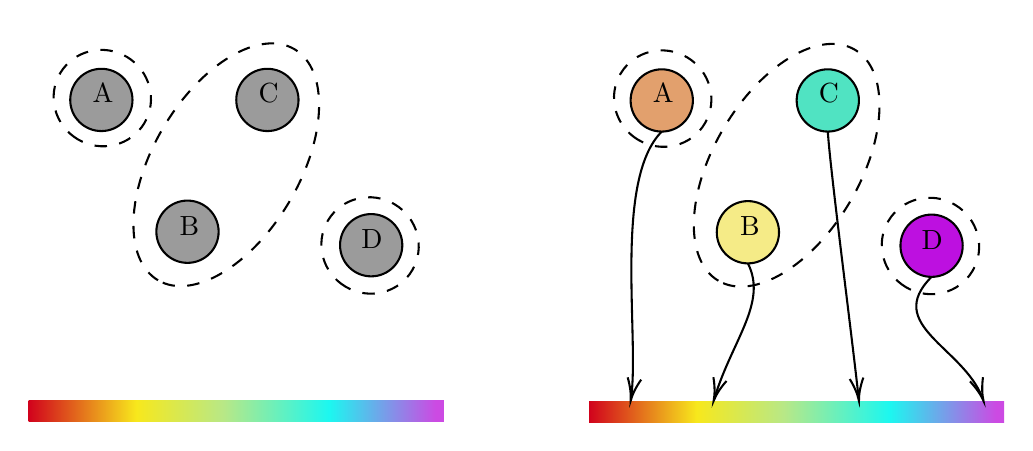
\begin{tikzpicture}[x=0.75pt,y=0.75pt,yscale=-1,xscale=1]
		%uncomment if require: \path (0,300); %set diagram left start at 0, and has height of 300
		
		%Shape: Circle [id:dp33643947845182054] 
		\draw  [fill={rgb, 255:red, 155; green, 155; blue, 155 }  ,fill opacity=1 ] (40,45) .. controls (40,36.72) and (46.72,30) .. (55,30) .. controls (63.28,30) and (70,36.72) .. (70,45) .. controls (70,53.28) and (63.28,60) .. (55,60) .. controls (46.72,60) and (40,53.28) .. (40,45) -- cycle ;
		%Shape: Circle [id:dp0443477789203186] 
		\draw  [fill={rgb, 255:red, 155; green, 155; blue, 155 }  ,fill opacity=1 ] (120,45) .. controls (120,36.72) and (126.72,30) .. (135,30) .. controls (143.28,30) and (150,36.72) .. (150,45) .. controls (150,53.28) and (143.28,60) .. (135,60) .. controls (126.72,60) and (120,53.28) .. (120,45) -- cycle ;
		%Shape: Circle [id:dp9214696658988042] 
		\draw  [fill={rgb, 255:red, 155; green, 155; blue, 155 }  ,fill opacity=1 ] (81.5,108.5) .. controls (81.5,100.22) and (88.22,93.5) .. (96.5,93.5) .. controls (104.78,93.5) and (111.5,100.22) .. (111.5,108.5) .. controls (111.5,116.78) and (104.78,123.5) .. (96.5,123.5) .. controls (88.22,123.5) and (81.5,116.78) .. (81.5,108.5) -- cycle ;
		%Shape: Circle [id:dp13696565141434136] 
		\draw  [fill={rgb, 255:red, 155; green, 155; blue, 155 }  ,fill opacity=1 ] (170,115) .. controls (170,106.72) and (176.72,100) .. (185,100) .. controls (193.28,100) and (200,106.72) .. (200,115) .. controls (200,123.28) and (193.28,130) .. (185,130) .. controls (176.72,130) and (170,123.28) .. (170,115) -- cycle ;
		%Shape: Ellipse [id:dp12864986832842984] 
		\draw  [dash pattern={on 4.5pt off 4.5pt}] (82.3,131.88) .. controls (65.55,121.98) and (66.7,89.04) .. (84.86,58.31) .. controls (103.02,27.58) and (131.32,10.69) .. (148.06,20.58) .. controls (164.81,30.48) and (163.66,63.42) .. (145.5,94.15) .. controls (127.34,124.88) and (99.05,141.77) .. (82.3,131.88) -- cycle ;
		%Shape: Ellipse [id:dp1610627082678362] 
		\draw  [dash pattern={on 4.5pt off 4.5pt}] (43.7,64) .. controls (32.49,57.38) and (28.66,43.1) .. (35.16,32.12) .. controls (41.65,21.13) and (56,17.6) .. (67.21,24.22) .. controls (78.42,30.85) and (82.25,45.12) .. (75.75,56.11) .. controls (69.26,67.09) and (54.91,70.63) .. (43.7,64) -- cycle ;
		%Shape: Ellipse [id:dp12974777917337055] 
		\draw  [dash pattern={on 4.5pt off 4.5pt}] (172.7,135) .. controls (161.49,128.38) and (157.66,114.1) .. (164.16,103.12) .. controls (170.65,92.13) and (185,88.6) .. (196.21,95.22) .. controls (207.42,101.85) and (211.25,116.12) .. (204.75,127.11) .. controls (198.26,138.09) and (183.91,141.63) .. (172.7,135) -- cycle ;
		%Shape: Rectangle [id:dp6743641105872487] 
		\draw  [draw opacity=0][shading=_msh882t58,_3sybf9svc] (20,200.03) -- (20,190) -- (220,190) -- (220,200.03) -- cycle ;
		%Shape: Circle [id:dp41982950014639475] 
		\draw  [fill={rgb, 255:red, 226; green, 160; blue, 109 }  ,fill opacity=1 ] (310,45.25) .. controls (310,36.96) and (316.71,30.25) .. (325,30.25) .. controls (333.28,30.25) and (340,36.96) .. (340,45.25) .. controls (340,53.53) and (333.28,60.25) .. (325,60.25) .. controls (316.71,60.25) and (310,53.53) .. (310,45.25) -- cycle ;
		%Shape: Circle [id:dp8259512278629788] 
		\draw  [fill={rgb, 255:red, 80; green, 227; blue, 194 }  ,fill opacity=1 ] (390,45.25) .. controls (390,36.96) and (396.71,30.25) .. (405,30.25) .. controls (413.28,30.25) and (420,36.96) .. (420,45.25) .. controls (420,53.53) and (413.28,60.25) .. (405,60.25) .. controls (396.71,60.25) and (390,53.53) .. (390,45.25) -- cycle ;
		%Shape: Circle [id:dp07277556260180118] 
		\draw  [fill={rgb, 255:red, 245; green, 235; blue, 135 }  ,fill opacity=1 ] (351.5,108.75) .. controls (351.5,100.46) and (358.21,93.75) .. (366.5,93.75) .. controls (374.78,93.75) and (381.5,100.46) .. (381.5,108.75) .. controls (381.5,117.03) and (374.78,123.75) .. (366.5,123.75) .. controls (358.21,123.75) and (351.5,117.03) .. (351.5,108.75) -- cycle ;
		%Shape: Circle [id:dp6294612143917628] 
		\draw  [fill={rgb, 255:red, 189; green, 16; blue, 224 }  ,fill opacity=1 ] (440,115.25) .. controls (440,106.96) and (446.71,100.25) .. (455,100.25) .. controls (463.28,100.25) and (470,106.96) .. (470,115.25) .. controls (470,123.53) and (463.28,130.25) .. (455,130.25) .. controls (446.71,130.25) and (440,123.53) .. (440,115.25) -- cycle ;
		%Shape: Ellipse [id:dp7357850148564777] 
		\draw  [dash pattern={on 4.5pt off 4.5pt}] (352.29,132.12) .. controls (335.55,122.23) and (336.69,89.29) .. (354.85,58.56) .. controls (373.02,27.82) and (401.31,10.93) .. (418.06,20.83) .. controls (434.81,30.73) and (433.66,63.66) .. (415.5,94.39) .. controls (397.34,125.13) and (369.04,142.02) .. (352.29,132.12) -- cycle ;
		%Shape: Ellipse [id:dp5587385382701016] 
		\draw  [dash pattern={on 4.5pt off 4.5pt}] (313.7,64.25) .. controls (302.49,57.63) and (298.66,43.35) .. (305.15,32.36) .. controls (311.64,21.38) and (325.99,17.84) .. (337.21,24.47) .. controls (348.42,31.09) and (352.24,45.37) .. (345.75,56.35) .. controls (339.26,67.34) and (324.91,70.88) .. (313.7,64.25) -- cycle ;
		%Shape: Ellipse [id:dp4946869974787813] 
		\draw  [dash pattern={on 4.5pt off 4.5pt}] (442.7,135.25) .. controls (431.49,128.63) and (427.66,114.35) .. (434.15,103.36) .. controls (440.64,92.38) and (454.99,88.84) .. (466.21,95.47) .. controls (477.42,102.09) and (481.24,116.37) .. (474.75,127.35) .. controls (468.26,138.34) and (453.91,141.88) .. (442.7,135.25) -- cycle ;
		%Shape: Rectangle [id:dp7288880698372671] 
		\draw  [draw opacity=0][shading=_2kvz2ka7v,_s6rolseyi] (290,200.28) -- (290,190.25) -- (490,190.25) -- (490,200.28) -- cycle ;
		%Curve Lines [id:da9868746504728607] 
		\draw    (325,60.25) .. controls (301.72,83.52) and (314.22,158.9) .. (310.26,188.26) ;
		\draw [shift={(310,190)}, rotate = 279.63] [color={rgb, 255:red, 0; green, 0; blue, 0 }  ][line width=0.75]    (10.93,-3.29) .. controls (6.95,-1.4) and (3.31,-0.3) .. (0,0) .. controls (3.31,0.3) and (6.95,1.4) .. (10.93,3.29)   ;
		%Curve Lines [id:da6841947081825557] 
		\draw    (455,130.25) .. controls (431.72,153.52) and (470.16,164.07) .. (479.47,188.49) ;
		\draw [shift={(480,190)}, rotate = 252.07] [color={rgb, 255:red, 0; green, 0; blue, 0 }  ][line width=0.75]    (10.93,-3.29) .. controls (6.95,-1.4) and (3.31,-0.3) .. (0,0) .. controls (3.31,0.3) and (6.95,1.4) .. (10.93,3.29)   ;
		%Curve Lines [id:da5128158053664607] 
		\draw    (366.5,123.75) .. controls (376.05,142.61) and (358.96,160.76) .. (350.51,188.3) ;
		\draw [shift={(350,190)}, rotate = 286.14] [color={rgb, 255:red, 0; green, 0; blue, 0 }  ][line width=0.75]    (10.93,-3.29) .. controls (6.95,-1.4) and (3.31,-0.3) .. (0,0) .. controls (3.31,0.3) and (6.95,1.4) .. (10.93,3.29)   ;
		%Curve Lines [id:da01085903440845759] 
		\draw    (405,60.25) .. controls (406.22,79.11) and (416.33,156.32) .. (419.8,188.11) ;
		\draw [shift={(420,190)}, rotate = 263.92] [color={rgb, 255:red, 0; green, 0; blue, 0 }  ][line width=0.75]    (10.93,-3.29) .. controls (6.95,-1.4) and (3.31,-0.3) .. (0,0) .. controls (3.31,0.3) and (6.95,1.4) .. (10.93,3.29)   ;
		
		% Text Node
		\draw (49.25,35.5) node [anchor=north west][inner sep=0.75pt]   [align=left] {A};
		% Text Node
		\draw (91.25,99.5) node [anchor=north west][inner sep=0.75pt]   [align=left] {B};
		% Text Node
		\draw (129.25,35.5) node [anchor=north west][inner sep=0.75pt]   [align=left] {C};
		% Text Node
		\draw (178.75,106) node [anchor=north west][inner sep=0.75pt]   [align=left] {D};
		% Text Node
		\draw (319.25,35.75) node [anchor=north west][inner sep=0.75pt]   [align=left] {A};
		% Text Node
		\draw (361.25,99.75) node [anchor=north west][inner sep=0.75pt]   [align=left] {B};
		% Text Node
		\draw (399.25,35.75) node [anchor=north west][inner sep=0.75pt]   [align=left] {C};
		% Text Node
		\draw (448.75,106.25) node [anchor=north west][inner sep=0.75pt]   [align=left] {D};
		
		
	\end{tikzpicture}
\end{figure}